\documentclass[Lau, oneside]{sapthesis}%remove "english" for a thesis written in Italian
%Bachelor's (laurea triennale) thesis : Lau 
%Master's (laurea specialistica) thesis: LaM 
%PhD's thesis: PhD 
\usepackage[italian]{babel} %use this package for a thesis written in Italian
\usepackage[utf8]{inputenx}
\usepackage{indentfirst}
\usepackage{microtype}
%\usepackage{chemformula}
%\usepackage{setspace}
%\usepackage{yfonts,color}
%\usepackage{siunitx}
%\usepackage{comment}
%\usepackage{multirow}
%\usepackage{varioref}
%\usepackage[bottom]{footmisc}
%\usepackage{wrapfig}
%\usepackage{float}
%\usepackage{type1cm}
\usepackage{lettrine}
\linespread{0.9}
%\usepackage{chngcntr}
\usepackage[nottoc, notlof, notlot]{tocbibind}
%\onehalfspacing
%\counterwithout{footnote}{chapter}
\usepackage{hyperref}
\hypersetup{
			hyperfootnotes=true,			
			bookmarks=true,			
			colorlinks=true,
			linkcolor=red,
                        linktoc=page,
			anchorcolor=black,
			citecolor=red,
			urlcolor=blue,
			pdftitle={A sample Bachelor's thesis for Sapienza Università di Roma},
			pdfauthor={FirstName LastName},
			pdfkeywords={thesis, sapienza, roma, university}
}

\title{Scheduler dei processi di un sistema operativo, confronto ed analisi di varie politiche}
\author{Simone Trenta}
\IDnumber{1724141}
\course[]{Ingegneria informatica ed automatica}
\courseorganizer{Facolt\`a di Ingegneria dell'informazione, informatica e statistica}
\submitdate{2020/2021}
\copyyear{2020}
\advisor{Prof. Giorgio Grisetti}
\authoremail{trenta.1724141@studenti.uniroma1.it}
\examdate{22 September 2015}
\examiner{Prof. ...} \examiner{Prof. ...} \examiner{Prof. ...}  \examiner{Prof. ...}  \examiner{Prof. ...} \examiner{Prof. ...}  \examiner{Prof. ...} 

%we refer to http://ctan.mirrorcatalogs.com/macros/latex/contrib/sapthesis/sapthesis-doc.pdf for an exhaustive description of the sapthesis documentclass.


\begin{document}

\frontmatter
\maketitle

\begin{abstract}
Tramite un progetto di simulazione di uno scheduler di un sistema operativo, si analizzano le varie politiche di scheduling fra le più comuni, ossia first came first served (FCFS), round robin (RR), shortest job first (SJF) e shortest remaining job first (SRJF).
\end{abstract}

\tableofcontents

\mainmatter
\chapter{Introduzione}
\lettrine[lines=2, findent=3pt, nindent=0pt]{I}{}n un sistema operativo la gestione delle richieste di risorse da parte dei processi è demandata allo scheduler.
Questa funzione di un sistema operativo è pressoché essenziale, senza la quale le risorse disponibili non potrebbero essere riservate e utilizzate in modo efficiente.

\bigskip
Nel \hyperref[chap:1]{Capitolo~\ref*{chap:1}}

\bigskip
Nel \hyperref[chap:2]{Capitolo~\ref*{chap:2}} 

\bigskip
Nel \hyperref[chap:3]{Capitolo~\ref*{chap:3}} 

\chapter{Lo scheduler in un sistema operativo}
\label{chap:1} 
\section{La sua utilità}
\label{sec:utilita}
Un odierno sistema operativo è composto da molteplici parti, una di esse è lo scheduler dei processi.
Questi ultimi sono parte costituente del sistema operativo, sono la parte esecutiva di esso.
Per meglio capire, i processi richiedono delle risorse del calcolatore, che siano risorse unicamente della CPU oppure di risorse di I/O.
Qualunque tipo di risorsa richiedano, spesso non è immediatamente disponibile, essendo limitate in un calcolatore.
Per cui è necessaria la presenza di un elemento che permetta al dispositivo di gestire le proprie risorse, tale elemento è per l'appunto lo scheduler.
Vedendo il problema da parte dei processi, problema che è la possibilità di usare una risorsa o meno, si crea la necessità di dare delle priorità per poterne usufruire.
Andando quindi a dare origine a tali priorità si producono di conseguenza delle politiche per poterle mettere in atto.

\section{Politiche di scheduling}
\label{sec:politiche}
Le politiche di scheduling sono degli algoritmi, che permettono quindi di riservare le risorse del calcolatore in un certo modo.
Ognuna di esse ha, come ogni cosa, dei vantaggi e degli svantaggi.
Tale prospettiva non permette di rendere efficiente una unica politica per ogni tipo di calcolatore, ma sarà necessario dotare ogni sistema operativo con l'algoritmo più adatto.
Alcuni parametri che vengono persi in considerazione per valutare l'efficienza di un algoritmo sono:
\begin{itemize}
\item Utilizzo della CPU
\item Throughput del sistema
\item Tempo di attesa di un processo
\item Turnaround di un processo
\item tempo di risposta di un processo
\end{itemize}
Fra questi non tutti potranno essere ottimizzati allo stesso tempo, in particolare nei sistemi batch si massimizza throughput e minimizza il turnaround, mentre nei sistemi interattivi si minimizza il tempo medio di risposta ed il tempo di attesa.
I parametri considerati nel progetto implementato sono il tempo di attesa e il tempo di completamento di un processo.
Quest'ultimo da considerarsi come il tempo totale che ogni processo ha impiegato per terminare, per cui partendo sempre dallo stesso valore per il tempo massimo iniziale, se il tempo di completamento sarà elevato vorrà dire che il processo ha impiegato molto per concludersi, rimanendo talvolta in attesa.

\subsection{First came first served}
\label{ssec:fcfs}
L'algoritmo \textit{first came first served}, forse, è il più semplice da capire, e da implementare.
Come dice il nome stesso esso non ha una particolare complessità, semplicemente quando un processo arriva, se è disponibile la risorsa, quindi un core della cpu, esso viene messo in running.
Altrimenti viene messo in una coda di waiting, dalla quale vengono presi i processi da mettere in running, prima di considerare i nuovi processi in arrivo.
In questa politica può risultare che un processo debba attendere la terminazione di un altro prima di poter entrare in running.
Per cui può risultare che dovrà attendere molto in stato di waiting, nascendo quindi il problema di attesa lunghe se le durate dei processi sono elevate.

\subsection{Round robin}
\label{ssec:rr}
L'algoritmo \textit{round robin} è una successiva perfezione del precedente fcfs (first came first served).
Anche in questo caso è presente una coda dei processi che sono arrivati.
Se è disponibile la risorsa richiesta dal processo in arrivo, gli viene riservata e tale processo può sfruttarla, altrimenti viene inserito nella coda di attesa.
Un processo in running, però, non ha la risorsa riservata fino a quando lo necessita, ma in questo caso è presente un clock, che inizia a scorre appena il processo entra in running.
Terminato il clock, la risorsa viene liberata dal processo.
Esso viene inserito nella coda dei processi in attesa, e da essa viene preso il primo processo per destinargli la risorsa appena liberatesi.
Il problema di questo algoritmo è scegliere un valore ottimale per il clock, se troppo elevato si tenderà ad avere un approccio simile a fcfs, se non uguale, se troppo breve i processi non riusciranno a sfruttare la risorsa richiesta che dovranno liberarla.

\subsection{Shortest job first}
\label{ssec:sjf}
L'algoritmo \textit{shortest job first} ordina i processi da mettere in running, ovviamente se c'è disponibilità di risorsa, in base a quanto tempo essi la richiedono, dal più breve al più lungo.
Anche in questo algoritmo un processo entrato in running termina completamente il suo job prima di terminare.
Se la risorsa non è disponibile, il processo viene inserito in una coda, il cui ordinamento è basato sulla durata del job.
Inoltre tutti i processi da mettere in running vengono presi da questa coda a cui si aggiungo i processi che arrivano in un determinato istante.
In questo algoritmo risulterà che i processi con la richiesta minore di risorsa saranno schedulati e termineranno per primi.
Il tempo medio di attesa si riduce, però il problema principale di questa politica nella realtà è riuscire a predire, con sufficiente accuratezza, quanto un processo occuperà una risorsa.
Nel caso del simulatore sviluppato ciò non è necessario, poiché ogni processo che arriva dichiara per quanto tempo occuperà la risorsa.
Al contrario, realisticamente, si utilizza la seguente formula per predire l'utilizzo successivo della cpu:
\begin{equation}\label{predizione}
   \hat{b}_{t+1} = \alpha b_t + (1 - \alpha) \hat{b}_t
\end{equation}
In cui si ha:
\begin{equation}
  \hat{b}_{t+1}
\end{equation}
è la predizione al tempo t+1;
\begin{equation}
    \alpha
\end{equation}
è il coefficiente di decadimento;
\begin{equation}
    b_t
\end{equation}
è la misura avvenuta al tempo t;
\begin{equation}
    \hat{b}_t
\end{equation}
è la predizione al tempo t.

\subsection{Shortest remaining job first}
\label{ssec:srjf}
L'algoritmo \textit{shortest remaining job first} è simile al precedente sjf.
Però in questo caso ad ogni ciclo di clock della cpu, i processi in running vengono confrontati con tutti quelli in waiting e quelli appena arrivati.
I processi, sempre in base alla disponibilità della risorsa, vengono messi in running, o ci rimangono, in ordine in base alla durata del job, dal più piccolo al più grande.
Anche in questo caso il problema principale è riuscire a predire la durata della richiesta della risorsa, e si utilizza la formula \eqref{predizione}.

\chapter{Sviluppo ed implementazione del simulatore}
\label{chap:2}
\section{Il progetto}
Il progetto sviluppato permette di simulare uno scheduler con le relative politiche presentate nella \hyperref[sec:politiche]{sezione~\ref*{sec:politiche}}.
L'implementazione è stata fatta usando il linguaggio di programmazione C, utilizzando il paradigma di programmazione funzionale con strutture dati create ad hoc. 
Per lo scopo sono state scritte varie librerie apposite, a seguire la spiegazione di ogni libreria, mentre per consultarle si può andare alla repository \hyperref[ref:repo]{[\ref*{ref:repo}]} dove, inoltre, è presente tutto il codice del progetto.

\section{Libreria process.h}
\label{sec:process.h}
Nella libreria \textit{process.h} \hyperref[ref:proch]{[\ref*{ref:proch}]} viene implementato un tipo di dato per simulare un processo.
Per poter fare ciò si è fatto uso di una struttura dati, con all'interno sia tipi di dati primitivi, che tipi di dato enumerati.
La struttura creata, chiamata \textit{ProcessType}, contiene al suo interno:
\begin{itemize}
    \item un intero, chiamato \textit{pid}, indicante il pid del processo simulato;
    \item un intero, chiamato \textit{time\_arrive}, indicante il tempo di arrivo;
    \item un intero, chiamato \textit{duration}, indicante la durata del job;
    \item un tipo di dato enumerato, chiamato \textit{ResourceType}, indicante che tipo di risorsa si richiede. Può assumere i valori 0, per chiedere risorse prettamente di CPU, oppure 1, indicante che oltre alla CPU ha una parte di interattività con l'utente, richiedendo risorse di tipo I/O;
    \item un tipo di dato enumerato, chiamato \textit{StateType}, indicante lo stato in cui si trova il processo. Può assumere i valori, 0 per lo stato NOT\_STATE, 1 per RUNNING, 2 per WAITING, 3 per READY, 4 per TERMINATED e 5 per BURST.
\end{itemize}

Lo stato NOT\_STATE indica che il processo è stato creato, ma ancora non è arrivato.
Lo stato RUNNING significa che il processo è in esecuzione, ha una risorsa riservata e sta procedendo.
Lo stato WAITING vuol dire che il processo non ha trovato risorse disponibili, è in attesa che se ne liberino.
Lo stato READY indica che il processo è appena arrivato e deve ancora essere schedulato.
Lo stato TERMINATED significa che il processo ha terminato completamente la sua esecuzione ed è uscito dallo scheduler.
Lo stato BURST, invece, vuol dire che il processo ha terminato una sua esecuzione, ma richiederà nuovamente delle risorse successivamente.

In tale libreria sono presenti funzioni per la gestione di tali processi.
Come funzioni per crearli partendo dai dati passati come parametri, per stamparli a video o in un file, controllare in che stato siano o che risorsa hanno richiesto, cambiarne lo stato ed anche richiedere un nuovo burst (nuova risorsa).
Quest'ultima funzione è particolarmente importante, in quanto permette al processo di richiedere una nuova risorsa, rimanendo così nel ciclo dello scheduler.
Ciò è implementato andando a generare numeri pseudo-casuali tramite la funzione di libreria standard \textit{rand}, opportunamente scalata su numeri adeguati, in base a ciò che si richiede.
Per un nuovo tipo di risorsa si scalerà i numeri in un range di 2, risultando i numeri calcolati o 0 o 1.
Per la durata del nuovo job, invece, si calcola come massimo il tempo medio voluto inizialmente, così che il job potrà durare da 0 al tempo medio.
Per il nuovo tempo di arrivo è calcolata partendo dal tempo attuale e come massimo il tempo massimo iniziale voluto moltiplicato per due.

\section{Libreria process\_list.h}
\label{sec:procList.h}
Nella libreria \textit{process\_list.h} \hyperref[ref:listproch]{[\ref*{ref:listproch}]} viene creata una lista concatenata di processi, con il tipo di dato spiegato nella \hyperref[sec:process.h]{sezione~\ref*{sec:process.h}}.
I suoi elementi sono strutture dati così composte:
\begin{itemize}
    \item un puntatore ad una struttura dati ProcessType, in cui sono contenute tutte le informazioni del processo in lista;
    \item un puntatore all'elemento successivo.
\end{itemize}
Tale struttura dati prende il nome di \textit{ProcessItem}.
La struttura dati rappresentante la lista concatenata è costituita da 2 elementi:
\begin{itemize}
    \item un intero, chiamato \textit{size}, indicante la dimensione della lista, ossia quanti processi ci sono in essa;
    \item un puntatore ad un dato ProcessItem, il quale è il primo elemento della lista.
\end{itemize}

In questa libreria sono presenti funzioni per una lista partendo dai dati letti da un file, per stamparla a video o in un file, contare i numeri di processi che sono in un determinato stato, generare una nuova richiesta di burst per i processi che ne sono in condizione.
Di queste funzioni una importante è quella che permette di inserire un nuovo elemento nella lista.
Tale funzione lo inserisce in testa, permettendo quindi di avere un costo costante pari a O(1), soluzione ottima per l'inserimento degli elementi in una lista.

Inoltre ci sono funzioni per la gestione delle statistiche, aggiornamento tempi di attesa e di completamento, che grazie al tipo di dato ed ad altre funzioni implementate nella libreria descritta nella \hyperref[sec:stat.h]{sezione~\ref*{sec:stat.h}}, le tengono sempre aggiornate.

\section{Libreria setting.h}
\label{sec:setting.h}
La libreria \textit{setting.h} \hyperref[ref:settingh]{[\ref*{ref:settingh}]} permette di creare un tipo di dato contenente le impostazioni iniziali su cui far girare il simulatore.
Tale tipo di dato è una struttura chiamata \textit{SettingType} contenente al suo interno:
\begin{itemize}
    \item un intero, indicante il numero di core, chiamato \textit{core};
    \item un intero, indicante il numero di processi, chiamato \textit{pid};
    \item un intero, indicante il tempo medio del job dei processi, chiamato \textit{avg\_time};
    \item un intero, indicante il tempo massimo iniziale di arrivo dei processi e durante il quale ogni processo chiederà nuovi burst, chiamato \textit{max\_time}.
\end{itemize}

In questa libreria è implementata la funzione grazie alla quale vengono letti i dati in lista da un file e viene creato un puntatore ad un tipo di dato SettingType.
Inoltre è presente una funzione per stampare a video i dati contenuti in tale struttura.

\section{Libreria stat.h}
\label{sec:stat.h}
La libreria \textit{stat.h} \hyperref[ref:stath]{[\ref*{ref:stath}]} permette di gestire le statistiche createsi durante la simulazione.
Ciò avviene tramite una struttura che prende il nome di \textit{StatisticsType}, la quale è composta dai seguenti dati:
\begin{itemize}
    \item un intero, per indicare il numero di processi, chiamato \textit{num\_proc};
    \item un intero, indicante il numero di core, chiamato \textit{core};
    \item un array di interi, di grandezza num\_proc, per memorizzare il tempo di attesa di ogni singolo processo, chiamato \textit{waiting\_time};
    \item un array di interi, di grandezza num\_proc, per salvare in memoria il tempo in cui i processi sono rimasti nello scheduler, o anche il tempo totale di completamento di ogni singolo processo, chiamato \textit{completing\_time};
    \item un float, che indica il tempo medio di attesa di tutti i processi, chiamato \textit{medium\_wait\_time};
    \item un float, indicante il tempo medio di completamento di tutti i processi, chiamato \textit{medium\_complete\_time}.
\end{itemize}

Sono presenti funzioni, che oltre alla creazione della struttura dati, permettono di aggiornare le statistiche, calcolando la media dei tempi di attesa e completamento.
Sono implementate funzioni per la stampa a video e per il salvataggio in un file, quest'ultima ci permetterà poi di avere dati finali grazie ai quali potremo confrontare i vari algoritmi di scheduling implementati.

\section{Libreria utility.h}
\label{sec:label.h}
Con la libreria \textit{utility.h} \hyperref[ref:utilityh]{[\ref*{ref:utilityh}]} vengono implementate funzioni per l'utilizzo comune in più politiche di scheduling.
In particolare sono sviluppate funzioni per la gestione di un array di interi, il quale memorizzerà i pid dei vari processi, e sarà gestito secondo l'algoritmo specifico da implementare.
Inoltre sono presenti funzioni per la determinazione della durata iniziale dei job dei processi, che viene richiesto abbiano una durata media desiderata.

\section{Libreria macro.h}
\label{sec:macro.h}
L'ultima libreria prima di passare alle librerie in cui vengono implementati gli algoritmi di scheduling è la libreria \textit{macro.h} \hyperref[ref:macroh]{[\ref*{ref:macroh}]}.
In questa libreria non sono presenti funzioni, ma vengono unicamente definite macro di utilizzo globale nel simulatore, come i file da cui leggere i dati, e dove scrivere le statistiche finali create.
Sono presenti anche definizioni per richiamare le varie librerie fin'ora descritte e tutte le successive in cui ci sono le politiche di scheduling.
Per finire ci sono anche delle variabili numeriche per la definizioni del numero complessivo di set utilizzati, del numero di cicli per cui il simulatore finale dovrà girare ed anche il quanto di tempo utilizzato in RR.

\section{Libreria fcfs.h}
\label{sec:fcfs.h}
Iniziamo con la libreria \textit{fcfs.h} \hyperref[ref:fcfsh]{[\ref*{ref:fcfsh}]} a descrivere le varie implementazioni degli algoritmi di scheduling, riprendendo l'ordine in cui sono stati presentati nella \hyperref[sec:politiche]{sezione~\ref*{sec:politiche}}.
Per cui la prima politica sarà first came first served.
Per meglio descrivere la sua implementazione faremo riferimento al seguente schema a stati finiti.
\begin{figure}[h]
  \centering
  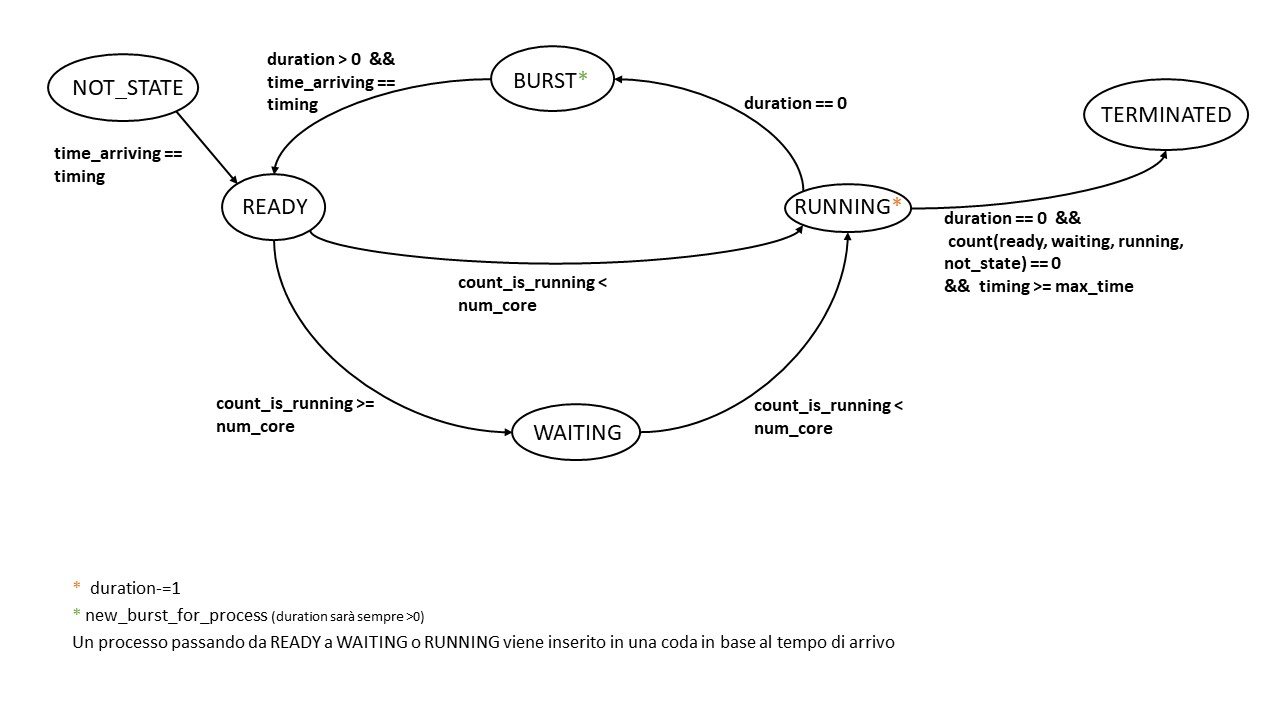
\includegraphics[width=1\textwidth]{schema a stati finiti FCFS.JPG}
  \caption{Schema a stati finiti FCFS}
\end{figure}

Ogni processo simulato (da ora in avanti per non appesantire la scrittura sarà denominato semplicemente processo, ma si intenderà sempre simulato) appena creato si trova nello stato NOT\_STATE.
Viene inserito in una lista con tutti i processi, viene creato un array contenente i pid dei processi che arriveranno.
Il simulatore inizia il suo percorso, andando a procedere per ogni singolo clock del processore (anche questo simulato), chiamato \textit{timing}.
Ad ogni clock si controlla nella lista i processi che hanno tempo di arrivo uguale a timing, nel qual caso si cambia il loro stato in READY.
Dopo di ciò, per tutti i processi in stato READY ed in stato di WAITING, quest'ultimi già in coda, e con precedenza a questi, se è disponibile la risorsa, quindi un core, il processo va in stato RUNNING.
Si contano nuovamente i processi in RUNNING, se tale numero è minore del numero di core disponibili, si procede ad inserire il successivo processo da READY a RUNNING.
Altrimenti, se non c'è più disponibilità di risorse, tutti i processi vengono inseriti in una coda in base al tempo di arrivo e il loro stato cambia in WAITING.
Ogni processo in RUNNING diminuisce di una unità la durata del suo job ad ogni ciclo di clock.
Quando la durata è uguale a 0, il processo cambia stato passando in BURST, liberando anche una risorsa.
In tale stato al processo vengono assegnati nuovi tempi di arrivo, nuova risorsa, nuova durata del job, grazie alla funzione descritta fine \hyperref[sec:process.h]{sezione~\ref*{sec:process.h}}.
Quando timing sarà uguale max\_time, descritto nella \hyperref[sec:setting.h]{sezione~\ref*{sec:setting.h}}, si passa ad un ciclo in cui i processi procedono come sopra descritto, ma quando il job sarà uguale a 0 non andranno in BURST, ma passeranno in TERMINATED, non richiedendo ulteriori risorse.
Una volta che tutti i processi in lista sono TERMINATED il simulatore con politica FCFS termina.
Ad ogni ciclo di clock, vengono sempre aggiornate le statistiche, per poi essere scritte in un file a terminazione della simulazione.

\section{Libreria rr.h}
\label{sec:rr.h}
La libreria \textit{rr.h} \hyperref[ref:rrh]{[\ref*{ref:rrh}]} implementa l'algoritmo round robin.
Prima di procedere all'analisi degli stati dei processi, in questa libreria viene implementato un ulteriore tipo di dato come struttura, per gestire i core ed il loro tempo ancora disponibile se utilizzati.
Tale struttura dati contiene:
\begin{itemize}
    \item un intero, indicante il pid del processo che sta utilizzando il core, chiamato \textit{pid};
    \item un intero, indicante il tempo rimanente per l'uso del core, chiamato \textit{core\_time}.
\end{itemize}
Prendendo in considerazione lo schema a stati finiti della seguente immagine analizziamo gli stati dei processi.
\begin{figure}[h]
  \centering
  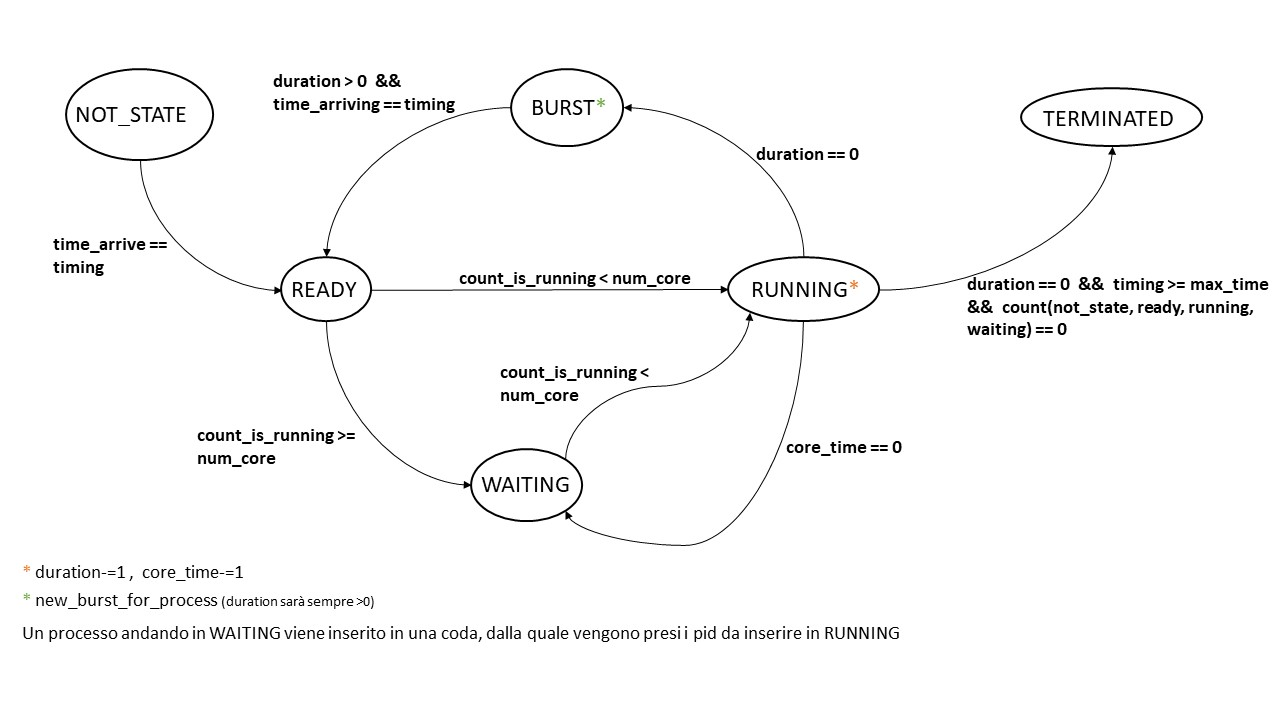
\includegraphics[width=1\textwidth]{schema a stati finiti RR.JPG}
  \caption{Schema a stati finiti RR}
\end{figure}

Ogni singolo processo appena creato si trova in stato NOT\_STATE e viene inserito nella lista dei processi.
Il simulatore inizia il suo primo ciclo, ad ogni clock cerca nella lista dei processi quelli per cui time\_arrive è uguale a timing.
Tali processi passano allo stato READY, essendo arrivati, e vengono inseriti in una coda per poterli gestire in base al loro arrivo.
Se è disponibile la risorsa, quindi il numero di processi in RUNNING  minore del numero di core, si prende il primo processo dalla coda e passa in RUNNING, reinizializzando il quanto del core al tempo prestabilito.
Si procede così fino a quando non terminano i core.
Tutti i rimanenti processi nella coda passano nello stato di WAITING.
Per tutti i processi in RUNNING viene ridotta di una unità la durata del job e del tempo rimanente del core.
Quando il core\_time è uguale a zero il processo passa nella coda dei processi in WAITING, e viene liberato un core, una risorsa.
Se invece la durata del job si riduce a zero il processo passa allo stato BURST.
In questo stato, come nella precedente politica, vengono calcolati nuovi tempi di arrivo, nuova durata del job e nuova richiesta di risorsa per il processo, come spiegato a fine \hyperref[sec:process.h]{sezione~\ref*{sec:process.h}}.
Quando il tempo trascorso nel primo ciclo del simulatore risulta maggiore di max\_time, si entra nell'ultimo ciclo, per cui il procedimento è come sopra descritto, ma quando un processo termina il job passa allo stato TERMINATED.
Quando tutti i processi sono nello stato TERMINATED il simulatore termina.
Ad ogni ciclo vengono aggiornate le statistiche, per poi essere scritte in un file, il quale è presente nella libreria macro.h, descritta nella \hyperref[sec:macro.h]{sezione~\ref*{sec:macro.h}}, a terminazione della simulazione.

\section{Libreria sjf.h}
\label{sec:sjf.h}
Proseguendo con l'analisi delle varie librerie in cui si implementano vari algoritmi di scheduling, la successiva è la libreria \textit{sjf.h} \hyperref[ref:sjfh]{[\ref*{ref:sjfh}]}.
Questa libreria implementa la politica di scheduling shortest job first.
Come per le precedenti librerie fcfs.h e rr.h, faremo riferimento al seguente schema a stati finiti per descrivere al meglio i passaggi fra stati in un processo.
\begin{figure}[h]
  \centering
  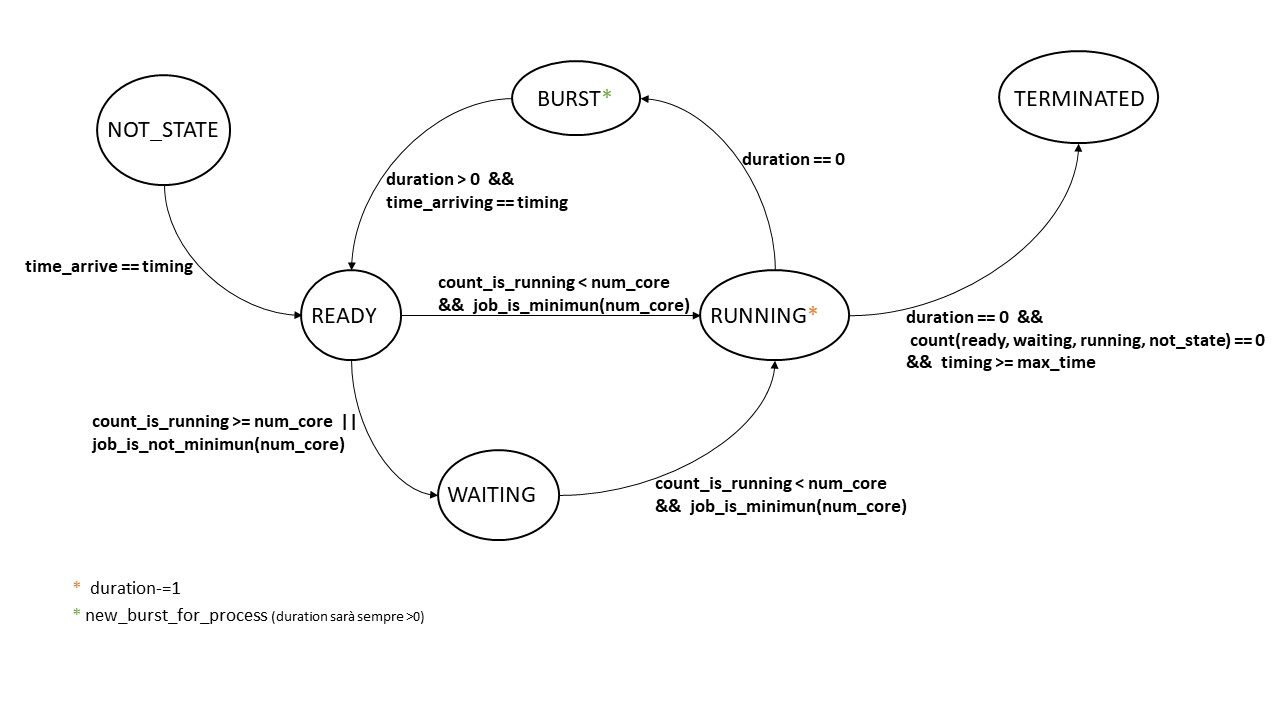
\includegraphics[width=1\textwidth]{schema a stati finiti SJF.jpg}
  \caption{Schema a stati finiti SJF}
\end{figure}

Come nei precedenti casi, ogni processo appena creato viene inserito in una lista dei processi e si trova nello stato NOT\_STATE.
Si procede con il primo del simulatore, fino a quando timing non raggiungerà max\_time.
Ad ogni clock si controlla la lista, se un processo ha il tempo di arrivo uguale a timing passerà in stato READY.
Per tutti i processi in READY e WAITING vengono fatti i seguenti due controlli per poter passare in RUNNING, i quali devono risultare entrambi positivi:
\begin{itemize}
    \item deve essere disponibile la risorsa richiesta, quindi in particolare almeno un core;
    \item la durata del job deve essere la minima fra tutti i processi in READY.
\end{itemize}
Come abbiamo detto nella \hyperref[ssec:sjf]{sezione~\ref*{ssec:sjf}}, il problema di questo algoritmo è prevedere la durata del job di ogni singolo processo in arrivo, questo poiché nella realtà i processi non dichiarano per quanto tempo occuperanno una risorsa.
Nel nostro caso, però, abbiamo fatto l'ipotesi che i processi lo dichiarino al loro arrivo.
Così facendo si implementa facilmente una funzione che permette di verificare se un processo ha la durata minima fra tutti quelli in READY.
Risultate positive entrambe le condizioni sopra descritte, il processo entra in RUNNING.
Altrimenti entra in WAITING.
Ogni processo in RUNNING diminuisce di una unità la durata rimanente del suo job ad ogni clock.
Quando la durata è uguale a zero il processo libera la risorsa fino ad allora occupa, ed entra in BURST.
In questo stato, come per i precedenti algoritmi, viene calcolato un nuovo tempo di arrivo, nuova durata del job ed una nuova richiesta di risorsa per il processo, come spiegato a fine \hyperref[sec:process.h]{sezione~\ref*{sec:process.h}}.
Una volta terminato il primo ciclo del simulatore, ossia quando timing risulta uguale max\_time, si entra nel secondo ciclo, ove il procedimento è lo stesso di quello sopra descritto.
Unica cosa che cambia è che ogni processo terminato il proprio job non va in BURST, ma bensì in TERMINATED, non richiedendo ulteriori risorse.
Quando tutti i processi saranno in TERMINATED il simulatore termina la sua esecuzione.
Ad ogni ciclo vengono inoltre aggiornate le statistiche per poi essere scritte in un file a termine dell'esecuzione.

\chapter{Esempi d'uso}
\label{chap:3}

\chapter{Conclusioni}
\label{chap:4}

\backmatter
\phantomsection
\begin{thebibliography}{17}

\bibitem{ref:repo}\label{ref:repo}
Repository github \url{https://github.com/simo-30/Relazione_finale_laurea_triennale}

\bibitem{ref:proch}\label{ref:proch}
Libreria process.h \url{https://github.com/simo-30/Relazione_finale_laurea_triennale/blob/master/codice/processo/process.h}

\bibitem{ref:listproch}\label{ref:listproch}
Liberia process\_list.h \url{https://github.com/simo-30/Relazione_finale_laurea_triennale/blob/master/codice/lista_processo/process_list.h}

\bibitem{ref:settingh}\label{ref:settingh}
Libreria setting.h \url{https://github.com/simo-30/Relazione_finale_laurea_triennale/blob/master/codice/setting/setting.h}

\bibitem{ref:stah}\label{ref:stath}
Libreria stat.h \url{https://github.com/simo-30/Relazione_finale_laurea_triennale/blob/master/codice/statistics/stat.h}

\bibitem{ref:utilityh}\label{ref:utilityh}
Libreria utility.h \url{https://github.com/simo-30/Relazione_finale_laurea_triennale/blob/master/codice/utility/utility.h}

\bibitem{ref:macroh}\label{ref:macroh}
Libreria macro.h \url{https://github.com/simo-30/Relazione_finale_laurea_triennale/blob/master/codice/utility/macro.h}

\bibitem{ref:fcfsh}\label{ref:fcfsh}
Libreria fcfs.h \url{https://github.com/simo-30/Relazione_finale_laurea_triennale/blob/master/codice/FCFS/fcfs.h}

\bibitem{ref:rrh}\label{ref:rrh}
Libreria rr.h \url{https://github.com/simo-30/Relazione_finale_laurea_triennale/blob/master/codice/RR/rr.h}

\bibitem{ref:sjfh}\label{ref:sjfh}
Libreria sjf.h \url{https://github.com/simo-30/Relazione_finale_laurea_triennale/blob/master/codice/SJF/sjf.h}

\end{thebibliography}

\end{document}